\documentclass[10pt]{amsart}

\usepackage{algorithm}
\usepackage[noend]{algpseudocode}
\usepackage{amsfonts}
\usepackage{amsmath}
\usepackage{amssymb}
\usepackage{amsthm}
\usepackage[backend=biber, citestyle=numeric-comp, bibstyle=ieee]{biblatex}
\usepackage{changepage}
\usepackage{enumitem}
\usepackage{fancyhdr}
\usepackage{fontspec}
\usepackage{fullpage}
\usepackage[hidelinks]{hyperref}
\usepackage{mathtools}
\usepackage{physics}
\usepackage[skins]{tcolorbox}
\usepackage{thmtools}
\usepackage{tikz}
\usepackage{tikz-3dplot}
\usetikzlibrary{angles, cd, quantikz, quotes, patterns}
\usepackage{titlesec}
\usepackage{wasysym}

\usepackage{tikz-cd}

\usepackage{bookmark}
\usepackage[nameinlink]{cleveref}

\titleformat{\section}[runin]{\normalsize\bfseries}{\thesection}{1em}{}[]
\titleformat{\subsection}[runin]{\normalsize\bfseries}{\thesubsection}{1em}{}[]
\titleformat{\subsubsection}[runin]{\normalsize\bfseries}{\thesubsubsection}{1em}{}[]

\addbibresource{solovay_kitaev_theorem.bib}

\theoremstyle{definition}
\newtheorem{theorem}{Theorem}
\newtheorem{definition}{Definition}
\theoremstyle{remark}
\newtheorem{problem}[theorem]{Problem}
\newtheorem{lemma}[theorem]{Lemma}
\newtheorem{remark}[theorem]{Remark}
\newtheorem{observation}[theorem]{Observation}
\newtheorem{example}[theorem]{Example}
\newtheorem{corollary}[theorem]{Corollary}

\renewcommand{\qedsymbol}{\(\blacksquare\)}

\setlength{\parindent}{0pt}

\DeclareMathOperator{\controrot}{CR}
\DeclareMathOperator{\expectation}{E}
\DeclareMathOperator{\gf}{GF}
\DeclareMathOperator{\qft}{QFT}
\DeclareMathOperator{\rk}{rk}
\DeclareMathOperator{\defect}{def}
\DeclareMathOperator{\swapgate}{SWAP}
\DeclareMathOperator{\che}{CHE}
\DeclareMathOperator{\poly}{poly}
\DeclareMathOperator{\Span}{Span}
\DeclareMathOperator{\diag}{diag}

\newcommand{\djk}{\delta_{j, k}}
\newcommand{\tlk}{\tilde{\lambda_k}}

\newcommand{\evalat}[2]{\left.{#1}\middle|\right._{#2}}

% SOURCE: https://tex.stackexchange.com/questions/296151/double-head-and-hook-arrow
\newcommand{\hookdoubleheadrightarrow}{%
  \hookrightarrow\mathrel{\mspace{-15mu}}\rightarrow
}

\newcommand{\draftcomment}[2]{\textcolor{#1}{#2}}

\newtcolorbox{edgebox}{enhanced, colback=white, frame code={%
\draw[very thin] (frame.north west) -- ($(frame.north west) + ( 0.5, 0)$);
\draw[very thin] (frame.north west) -- ($(frame.north west) + (0, -0.5)$);
\draw[very thin] (frame.south east) -- ($(frame.south east) + (-0.5, 0)$);
\draw[very thin] (frame.south east) -- ($(frame.south east) + (0,  0.5)$);
}}

\begin{document}
    \section*{The Solovay-Kitaev Theorem} \hfill \hfill valentinpi, Last Change: June 27, 2023

    \phantom{}

    Consider the following question: Given a finite set of \(1\)-qubit-gates, how fast can we approximate an arbitrary \(1\)-qubit-gate? A fundamental result is that a fast approximation is generally possible, as is established by the Solovay-Kitaev Theorem. In this note, we study a part of the proof following the version from Nielsen and Chuang and make some of the arguments more precise.

    \phantom{}

    The first reduction to make is to only consider \(\text{SU}(2)\). Due to the decomposition theorem of operators in \(\text{U}(2)\) into products of operators from \(\text{SU}(2)\) \cite[p. 176]{Nielsen}, this suffices. We shall recall that approximating general quantum gates is a hard problem \cite[pp. 198-200]{Nielsen}, as it can be shown that there are multi-qubit-gates, for which the complexity of approximation is exponentially lower bounded by the number of qubits. Since we are restricting ourselves to one qubit only however, this fact does not pose an issue.

    \phantom{}

    Let \(\mathcal{G} \subseteq \text{SU}(2)\) be a finite set, closed wrt. inverses meaning adjoints, s.t. \(\langle \mathcal{G} \rangle\) is dense in \(\text{SU}(2)\)  wrt. the trace distance \(d_{\tr}(A, B) = \trace(|A-B|) = \trace(\sqrt{(A-B)^\dagger(A-B)})\). Generally we may include \(E_2\) into \(\mathcal{G}\) to have a subgroup, but it suffices to leave it. Using the trace distance suffices as all norms in finite-dimensional spaces are equivalent. Let \(\mathcal{S}_{\varepsilon} \coloneqq d_{\tr}(\cdot, E_2)^{-1}([0, \varepsilon])\).

    \begin{figure}[!hbtp]
        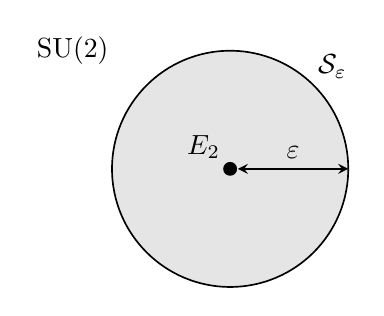
\begin{tikzpicture}[>=stealth, semithick]
            \tikzset{
                point/.style={circle, fill, inner sep=0pt, minimum size=5pt}
            };
            \draw[fill=black!10] (0, 0) circle (1.5cm);
            \node[point] (0) at (0, 0) {} node[above left] {\(E_2\)};
            \node at (1.3, 1.3) {\(\mathcal{S}_{\varepsilon}\)};
            \node at (-2, 1.5) {\(\text{SU}(2)\)};
            \draw[<->] (0) -- (1.5, 0) node[above, pos=0.5] {\(\varepsilon\)};
        \end{tikzpicture}
    \end{figure}

    \begin{lemma}[{\cite[pp. 619-623]{Nielsen}}] \label{net_lemma}
        There exists a universal constant \(\varepsilon_0 \in \mathbb{R}_{> 0}\), independent of \(\mathcal{G}\), s.t. for any \(\varepsilon \in \mathbb{R}\), \(\varepsilon \leq \varepsilon_0\), if \(\mathcal{G}^{\cdot \ell}\) with \(\ell \in \mathbb{N}\) is an \(\varepsilon^2\)-net for \(\mathcal{S}_{\varepsilon} \subseteq \text{SU}(2)\), then \(\mathcal{G}^{\cdot (5\ell)}\) is a \(C\varepsilon^3\)-net for \(\mathcal{S}_{\sqrt{C\varepsilon^3}}\), where \(C \in \mathbb{R}_{> 1}\), \(C \in \mathcal{O}(1)\).
    \end{lemma}

    \begin{figure}[!hbtp]
        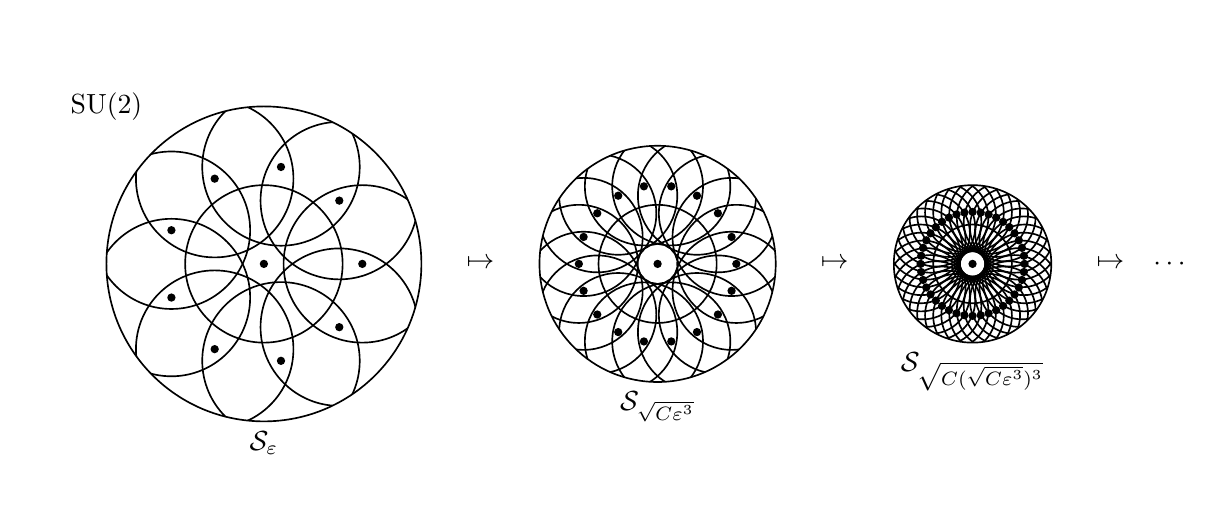
\begin{tikzpicture}[>=stealth, semithick]
            \tikzset{point/.style={circle, fill, inner sep=0pt, minimum size=3pt}};
            % First
            \node[point] (netpt) at (0, 0) {};
            \draw (netpt) circle (1cm);
            \foreach \a in {-4, ..., 4}{
                \node[point] (netpt) at (40*\a:1.25cm) {};
                \draw (netpt) circle (1cm);
            }
            \fill[even odd rule, white]
            (-3, -3) rectangle (3, 3)
            (0, 0) circle (2cm);
            \draw (0, 0) circle (2cm);
            \node at (-2, 2) {\(\text{SU}(2)\)};
            \node[below] at ($(0, 0) + (-90:2cm)$) {\(\mathcal{S}_{\varepsilon}\)};
            \node at (2.75, 0) {\(\mapsto\)};
            % Second
            \node[point] (netpt) at (5, 0) {};
            \draw (netpt) circle (0.75cm);
            \foreach \a in {-8, ..., 9}{
                \node[point] (netpt) at ($(5, 0) + (20*\a:1cm)$) {};
                \draw (netpt) circle (0.75cm);
            }
            \fill[even odd rule, white]
                (3, -2) rectangle (7, 2)
                (5, 0) circle (1.5cm);
            \draw (5, 0) circle (1.5cm);
            \node[below] at ($(5, 0) + (-90:1.5cm)$) {\(\mathcal{S}_{\sqrt{C\varepsilon^3}}\)};
            \node at (7.25, 0) {\(\mapsto\)};
            \node[point] (netpt) at (9, 0) {};
            \draw (netpt) circle (0.5cm);
            \foreach \a in {-19, ..., 20}{
                \node[point] (netpt) at ($(9, 0) + (9*\a:0.66cm)$) {};
                \draw (netpt) circle (0.5cm);
            }
            \fill[even odd rule, white]
                (7.5, -2) rectangle (10.5, 2)
                (9, 0) circle (1cm);
            \draw (9, 0) circle (1cm);
            \node at (10.75, 0) {\(\mapsto\)};
            \node at (11.5, 0) {\(\cdots\)};
            \node[below] at ($(9, 0) + (-90:1cm)$) {\(\mathcal{S}_{\sqrt{C(\sqrt{C\varepsilon^3})^3}}\)};
        \end{tikzpicture}
    \end{figure}

    \begin{theorem}[{Solovay-Kitaev Theorem \cite[pp. 618-620]{Nielsen}}]
         For any \(\varepsilon \in \mathbb{R}_{> 0}\), there exists an \(\ell \in \mathbb{N}\), \(\ell \in \mathcal{O}(\log_2^c(1/(C^2\varepsilon)))\) with \(c \in \mathbb{R}_{> 0}\), \(c \in \mathcal{O}(1)\) a universal constant, s.t. \(\mathcal{G}^{\cdot \ell}\) is an \(\varepsilon\)-net of \(\text{SU}(2)\).
    \end{theorem}

    \begin{proof}
        The first step is to prove that we can take an initial net and make it successively smaller with exponential speed. Take an arbitrary \(\varepsilon_0' \in (0, 1)\) with just \(\varepsilon_0' \leq \varepsilon_0\) for now. \(\langle \mathcal{G} \rangle\) is dense in \(\text{SU}(2)\), so there is an \(\varepsilon_0'^2\)-net of \(S_{\varepsilon_0'}\) by the following topological argument.

        \begin{edgebox}
            Since the determinant map \(\det\colon \mathbb{C}^{2 \times 2} \to \mathbb{C}\) is continuous as a polynomial and \(\text{SU}(2) = \det^{-1}(\{1\})\), \(\text{SU}(2)\) is closed in \(\mathbb{C}^{2 \times 2}\). The matrices being unitary gives the boundedness of \(\text{SU}(2) \subseteq \mathbb{C}^{2 \times 2} \cong \mathbb{R}^{8}\). Applying the Heine-Borel theorem gives the compactness of \(\text{SU}(2)\). To obtain an \(\varepsilon_0'^2\)-net for \(\text{SU}(2)\) and thus \(\mathcal{S}_{\varepsilon_0'}\), choose for any \(U \in \text{SU}(2)\) a \(V_U^{\ell_U} \in \mathcal{G}^{\cdot \ell_U} \subseteq \langle \mathcal{G} \rangle\) with \(\ell_U \in \mathbb{N}\), s.t. \(\norm*{U-V_U^{\ell_U}} < \varepsilon_0'^2\). Then \(\{V_U^{\ell_U}\}_{U \in \text{SU}(2)}\) is an open cover, so choose a finite cover \(\{V_1^{\ell_1}, ..., V_n^{\ell_n}\}\) with \(n \in \mathbb{N}_{\geq 1}\) and select \(\ell_0 \coloneqq \max\{\ell_1, ..., \ell_n\}\). We can do this analogously for \(\mathbb{S}_{\varepsilon_0'}\) to obtain a different \(\ell_0\) value and take the maximum.
        \end{edgebox}

        Apply the theorem on \(\mathcal{G}^{\cdot \ell_0}\) to obtain a \(C\varepsilon_0'^3\)-net of \(S_{\sqrt{C\varepsilon_0'^3}}\). Iterating \(k\)-times, \(k \in \mathbb{N}_{\geq 1}\), we obtain some \(\varepsilon_k\), which corresponds to applying the map \(\varepsilon \mapsto C^{1/2}\varepsilon^{3/2}\) exactly \(k\) times on \(\varepsilon_0'\). Looking at the exponents and considering \(\varepsilon_0' = C^0\varepsilon_0'^1\), we can alternatively consider the exponents as pairs and look at \(k\) applications of the map \((x, y) \mapsto (1/2+(3/2) x, (3/2) y)\) with initial values \((x, y) = (0, 1)\). For the first component we thus have the geometric sum
        \begin{align}
            \frac{1}{2} + \frac{3}{2}\left(\frac{1}{2} + \frac{3}{2}\left(...\left(\frac{1}{2} + \frac{3}{2}x\right)...\right)\right) &= \frac{1}{2} + \frac{3}{4} + \frac{9}{8} + \frac{27}{16} + \frac{81}{32} + ... + \frac{3^{k-1}}{2^k} + \frac{3^k}{2^k} x\\
            &= \frac{1}{3} \sum_{k'=0}^k \left(\frac{3}{2}\right)^{k'} - \frac{1}{3} + \left(\frac{3}{2}\right)^k x = \left(\frac{3}{2}\right)^k (x+1) - 1
        \end{align}
        for which the derivation may be visualized the following way.
        \begin{figure}[!hbtp]
            \begin{tikzpicture}[>=stealth, semithick]
                \node (00) at (0, 0) {\(\left(\frac{1}{2}\right.\)};
                \node[right=-0.1cm of 00] (01) {\(+\)};
                \node[right=-0.1cm of 01] (02) {\(\left.\frac{3}{2}\right)\)};
                \node[below=-0.1cm of 02] (10) {\(\cdot\)};
                \node[below=-0.1cm of 10] (00) {\(\left(\frac{1}{2}\right.\)};
                \node[right=-0.1cm of 00] (01) {\(+\)};
                \node[right=-0.1cm of 01] (22) {\(\left.\frac{3}{2}\right)\)};
                \node[below=-0.1cm of 22] (10) {\(\cdot\)};
                \node[below=-0.1cm of 10] (00) {\(\left(\frac{1}{2}\right.\)};
                \node[right=-0.1cm of 00] (01) {\(+\)};
                \node[right=-0.1cm of 01] (42) {\(\left.\frac{3}{2}\right)\)};
                \node[below=-0.1cm of 42] (10) {\(\cdot\)};
                \node[below=-0.1cm of 10] (00) {\(\left(\frac{1}{2}\right.\)};
                \node[right=-0.1cm of 00] (01) {\(+\)};
                \node[right=-0.1cm of 01] (62) {\(\left.\frac{3}{2}\right)\)};
                \node[below=-0.1cm of 62] (10) {\(\cdot\)};
                \node[below=-0.1cm of 10] (00) {\(\left(\frac{1}{2}\right.\)};
                \node[right=-0.1cm of 00] (01) {\(+\)};
                \node[right=-0.1cm of 01] (82) {\(\left.\frac{3}{2}\right)\)};
                \node[below=-0.1cm of 82] (10) {\(\cdot\)};
                \draw[->] (02) -- (22);
                \draw[->] (22) -- (42);
                \draw[->] (42) -- (62);
                \draw[->] (62) -- (82);
                \node[below=-0.1cm of 10] {\(x\)};
            \end{tikzpicture}
        \end{figure}
        In other words, \(\varepsilon_k = (C\varepsilon_0')^{((3/2)^k)}/C\) and \(\mathcal{G}^{\cdot 2^k \ell_0}\) is a \(\varepsilon_k^2\)-net of \(\mathcal{S}_{\varepsilon_k}\). Now assume \(C\varepsilon_0' \in (0, 1)\) to make the nets smaller with each increase of \(k\). Thus \(\varepsilon_k \to_{k \to \infty} 0\) under exponential decline. For the following, we want \(\varepsilon_k^2 < \varepsilon_{k+1}\) and the direct computation gives \(\varepsilon_0' \in (0, C)\) as a sufficient condition, so wlog. assume that.

        \phantom{}
        
        We now find an \(\ell\) as claimed by using the construction of nets from above. Let \(U \in \text{SU}(2)\) be arbitrary, but fixed and take a \(\varepsilon_0'^2\)-approximation of \(U\), denoted \(U_0 \in \mathcal{G}^{\cdot \ell_0}\). Set \(V_0 \coloneqq UU_0^\dagger\). Then
        \begin{align}
            d_{\tr}(V_0, E_2) = \tr|(U-U_0)U_0^\dagger| = \tr|U_0(U-U_0)U_0^\dagger| = \tr|U-U_0| = d_{\tr}(U, U_0) \leq \varepsilon_0^2 < \varepsilon_1
        \end{align}
        Establishing \(V_0 \in \mathcal{S}_{\varepsilon_1}\). By construction, \(\mathcal{G}^{\cdot (5 \ell_0)}\) is a \(\varepsilon_1^2\)-net of \(\mathcal{S}_{\varepsilon_1}\), so take an \(\varepsilon_1^2\)-approximation \(U_1 \in \mathcal{G}^{\cdot (5\ell_0)}\) of \(V_0\) and set \(V_1 \coloneqq V_0U_1^\dagger\). The same argument as before gives \(d_{\tr}(V_1, E_2) = d_{\tr}(U, U_1U_0) \leq \varepsilon_1^2 < \varepsilon_2\). We iterate this procedure to obtain for any \(k \in \mathbb{N}_{\geq 1}\) a unitary \(U_kU_{k-1}...U_0\) with \(U_i \in \mathcal{G}^{\cdot (5^i \ell_0)}\) for every \(i \in [0, k]_{\mathbb{N}}\), which is a \(\varepsilon_k^2\)-approximation of \(U\).
        \begin{figure}[!hbtp]
            \small
            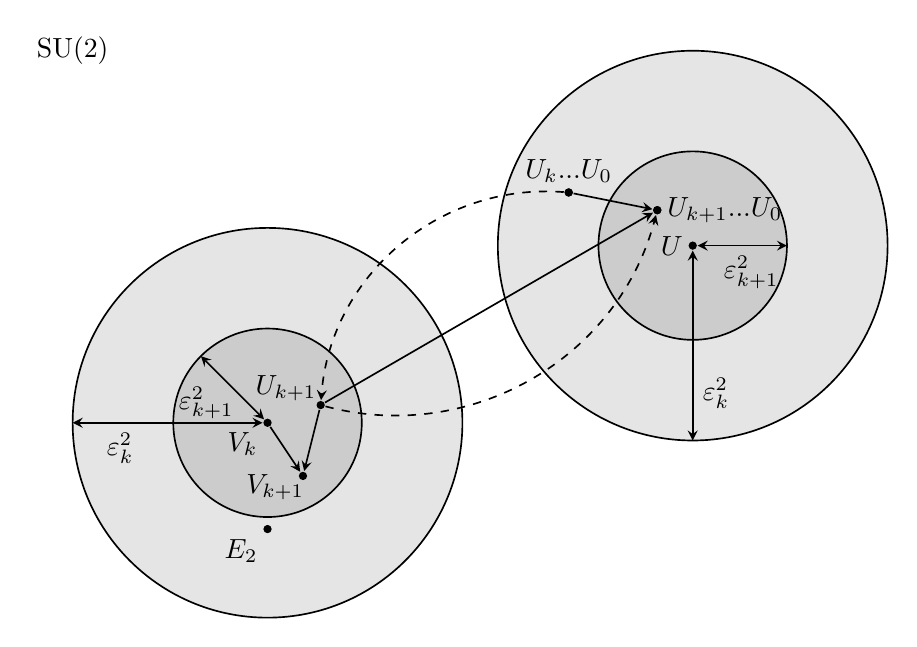
\begin{tikzpicture}[>=stealth, semithick, scale=0.9]
                \tikzset{point/.style={circle, fill, inner sep=0pt, minimum size=3pt}};
                \draw[fill=black!10] (0, 1.5) circle (2.75cm);
                \draw[fill=black!20] (0, 1.5) circle (1.33cm);
                \node[point] (Vkpt) at (0, 1.5) {};
                \node[below left] at (Vkpt) {\(V_k\)};
                \node[point] (E2pt) at (0, 0) {};
                \node[below left] at (E2pt) {\(E_2\)};
                \draw[fill=black!10] (6, 4) circle (2.75cm);
                \draw[fill=black!20] (6, 4) circle (1.33cm);
                \node[point] (Upt) at (6, 4) {};
                \node[left] at (Upt) {\(U\)};
                \draw[<->] (Upt) -- ($(Upt) + (-90:2.75cm)$) node[right, pos=0.75] {\(\varepsilon_k^2\)};
                \draw[<->] (Upt) -- ($(Upt) + (0:1.33cm)$) node[below, pos=0.6] {\(\varepsilon_{k+1}^2\)};
                \node[point] (kpt) at (4.25, 4.75) {};
                \node[point] (kp1pt) at (5.5, 4.5) {};
                \node[above] at (kpt) {\(U_k...U_0\)};
                \node[right] at (kp1pt) {\(U_{k+1}...U_0\)};
                \draw[->] (kpt) -- (kp1pt);
                \node[point] (kpt) at (4.25, 4.75) {};
                \node[point] (kp1pt) at (5.5, 4.5) {};
                \node[point] (Ukp1pt) at (0.75, 1.75) {};
                \node[above left=-0.1cm] at (Ukp1pt) {\(U_{k+1}\)};
                \draw[<->] (Vkpt) -- ($(Vkpt) + (180:2.75cm)$) node[below, pos=0.75] {\(\varepsilon_k^2\)};
                \draw[<->] (Vkpt) -- ($(Vkpt) + (135:1.33cm)$) node[below left=-0.2cm, pos=0.5] {\(\varepsilon_{k+1}^2\)};
                \draw[->] (Ukp1pt) -- (kp1pt);
                \node[point] (Vkp1pt) at (0.5, 0.75) {};
                \path[->] (Vkpt) edge (Vkp1pt) (Ukp1pt) edge (Vkp1pt);
                \node[below left=-0.2cm] at (Vkp1pt) {\(V_{k+1}\)};
                \node at (-2.75, 6.75) {\(\text{SU}(2)\)};
                \path[->, dashed] (kpt) edge[bend right=45] (Ukp1pt);
                \path[->, dashed] (Ukp1pt) edge[bend right=45] (kp1pt);
            \end{tikzpicture}
        \end{figure}

        \begin{edgebox}
            We used  the following properties of the trace from \cite[p. 75]{Nielsen} here: Consider that the trace \(\tr\) is \emph{additive} and \emph{cyclic}, in the sense that
            \begin{align}
                \tr(A+B) = \tr(A) + \tr(B) \text{ and } \tr(AB) = \tr(BA)
            \end{align}
            for any \(A, B \in \mathbb{C}^{n \times n}\), \(n \in \mathbb{N}_{\geq 1}\). Thus the trace is perserved under unitary transformations, meaning that for any \(U \in U(n)\),
            \begin{align}
                \tr(UAU^\dagger) = \tr(U^\dagger UA) = \tr(A)
            \end{align}
            is fulfilled.
        \end{edgebox}
        \begin{figure}[!hbtp]
            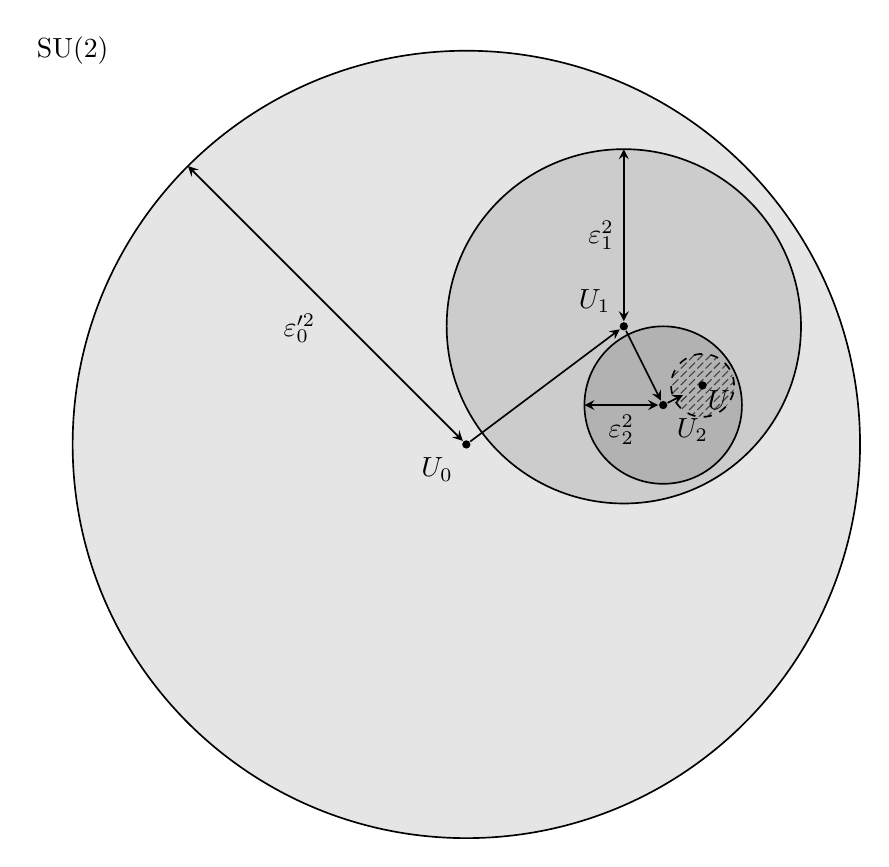
\begin{tikzpicture}[>=stealth, semithick]
                \tikzset{point/.style={circle, fill, inner sep=0pt, minimum size=3pt}};
                \draw[fill=black!10] (0, 0) circle (5cm);
                \draw[fill=black!20] (2, 1.5) circle (2.25cm);
                \draw[fill=black!30] (2.5, 0.5) circle (1cm);
                \node[point] (e0pt) at (0, 0) {};
                \node[below left=0cm of e0pt] {\(U_0\)};
                \node[point] (e1pt) at (2, 1.5) {};
                \node[above left=0cm of e1pt] {\(U_1\)};
                \node[point] (e2pt) at (2.5, 0.5) {};
                \node[below right=0cm of e2pt] {\(U_2\)};
                \fill[dashed, draw, pattern={north east lines}, pattern color=black!75] (3, 0.75) circle(0.4cm);
                \node[point] (Upt) at (3, 0.75) {};
                \node[below right=-0.15cm of Upt] {\(U\)};
                \draw[<->] (e0pt) -- ($(e0pt) + (135:5cm)$) node[below left, pos=0.5] {\(\varepsilon_0'^2\)};
                \draw[<->] (e1pt) -- ($(e1pt) + (90:2.25cm)$) node[left, pos=0.5] {\(\varepsilon_1^2\)};
                \draw[<->] (e2pt) -- ($(e2pt) + (180:1cm)$) node[below, pos=0.5] {\(\varepsilon_2^2\)};
                \node at (-5, 5) {\(\text{SU}(2)\)};
                \path[->] (e0pt) edge (e1pt) (e1pt) edge (e2pt);
                \draw[->] (e2pt) -- ($(e2pt)!0.5!(Upt)$);
            \end{tikzpicture}
        \end{figure}
        We require a total of \(\sum_{i=0}^k 5^i \ell_0 = \frac{5^{k+1}-1}{4}\ell_0 < 5/4 \cdot 5^k \ell_0\) gates. To approximate with a precision of \(\varepsilon\), we use the Ansatz \(\varepsilon_k^2 < \varepsilon\) and conclude
        \begin{align}
            \left(\frac{3}{2}\right)^k > \frac{1}{2}\frac{\log_2(C^2\varepsilon)}{\log_2(C\varepsilon_0')}
        \end{align}
        where we wlog. assume \(C^2\varepsilon \in (0, 1)\). Set \(c \coloneqq \log_{3/2}(5) = \log_2(5)/\log_2(3/2)\) and obtain a gate count of
        \begin{align}
            \frac{5}{4} 5^k \ell_0 = \frac{5}{4} \left(\frac{3}{2}\right)^{ck} \ell_0 \leq \frac{5}{4} \frac{1}{2^c}\frac{\log_2^c(C^2\varepsilon)}{\log_2^c(C\varepsilon_0')} \ell_0 \in \Theta(\log_2^c(1/(C^2\varepsilon)))
        \end{align}
        where we omit any rounding to a next number \(k\) sufficing the construction, proving the Solovay-Kitaev Theorem.
    \end{proof}

    \printbibliography{}
\end{document}
